\section{Classifying by Determinant}
\begin{frame}{THC-cromwell matrix}
	\begin{itemize}
		\item The \term{cromwell matrix} of a knot is an $n \times n$ binary matrix such that each row and column has exactly two $1$s.
		\item The \term{THC-cromwell matrix} is an expansion of cromwell matrix into $\theta$-curves and handcuff graphs that satisfies the following conditions :
		\begin{enumerate}
			\item It is a $(n+1)\times n$ bianry matrix.
			\item It contains exactly two $1$s in every column.
			\item There exists two distinct rows which contains exactly three $1$s, which is called the \term{three-row}. Every other row contains exactly two $1$s.
		\end{enumerate}
		$$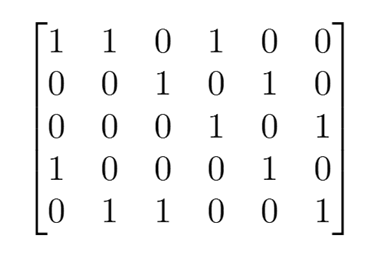
\includegraphics[width=.4\linewidth]{figure/cromwell.png}$$
	\end{itemize}
\end{frame}

\begin{frame}{Determinant of the cromwell matrices of Knot}
	\begin{thm}
		Let $K$ be any knot then its determinant of the cromwell matrix is $0$ or $\pm2$.
	\end{thm}
	\mypf
	\begin{tabu}{X[5c]X[c]X[5c]X[c]X[5c]}
			\raisebox{-1.5cm}{
\includegraphics[height=3cm]{figure/Trefoilimage.png}} &
			$\longmapsto$ &
			$\begin{bmatrix}
				\textcolor{red}{1} & 0 & \textcolor{red}{1} & 0 & 0\\
				0 & \textcolor{red}{1} & 0 & \textcolor{red}{1} & 0\\
				0 & 0 & \textcolor{red}{1} & 0 & \textcolor{red}{1}\\
				\textcolor{red}{1} & 0 & 0 & \textcolor{red}{1} & 0\\
				0 & \textcolor{red}{1} & 0 & 0 & \textcolor{red}{1}
			\end{bmatrix}$&
			$\longmapsto$ &
			$\begin{bmatrix}
				\textcolor{red}{1} & \textcolor{red}{1} & 0 & 0 & 0\\
				0 & \textcolor{red}{1} & \textcolor{red}{1} & 0 & 0\\
				0 & 0 & \textcolor{red}{1} & \textcolor{red}{1} & 0\\
				0 & 0 & 0 & \textcolor{red}{1} & \textcolor{red}{1}\\
				\textcolor{red}{1} & 0 & 0 & 0 & \textcolor{red}{1}
			\end{bmatrix}$
	\end{tabu}
\end{frame}
\begin{frame}
	\begin{enumerate}
		\item[\mybf{CASE 1.}] \mybf{When $n$ is an even number.}
	\end{enumerate}
	%\vspace*{-10pt}
	\begin{tabu}{X[5c]X[c]X[5c]X[c]X[5c]}
		$\begin{bmatrix}
			\textcolor{red}{1} & \textcolor{red}{1} & 0 & 0 \\
			0 & \textcolor{red}{1} & \textcolor{red}{1} & 0\\
			0 & 0 & \textcolor{red}{1} & \textcolor{red}{1}\\
			\textcolor{red}{1} & 0 & 0 & \textcolor{red}{1}
		\end{bmatrix}$ &
		$\longmapsto$ &
		$\begin{bmatrix}
			\textcolor{red}{1} & \textcolor{red}{1} & 0 & 0 \\
			0 & \textcolor{red}{1} & \textcolor{red}{1} & 0\\
			0 & 0 & \textcolor{red}{1} & \textcolor{red}{1}\\
			\textcolor{PineGreen}{2} & \textcolor{PineGreen}{2} & \textcolor{PineGreen}{2} & \textcolor{PineGreen}{2}
		\end{bmatrix}$ &
		$\longmapsto$ &
		$\begin{bmatrix}
			\textcolor{red}{1} & \textcolor{red}{1} & 0 & 0 \\
			0 & \textcolor{red}{1} & \textcolor{red}{1} & 0\\
			0 & 0 & \textcolor{red}{1} & \textcolor{red}{1}\\
			\textcolor{Aquamarine}{0} & \textcolor{Aquamarine}{0} & \textcolor{Aquamarine}{0} & \textcolor{Aquamarine}{0}
		\end{bmatrix}$ &
	\end{tabu}
	So the determinant of $K$ is $0$.
	\begin{enumerate}
		\item[\mybf{CASE 2.}] \mybf{When $n$ is an odd number.}
	\end{enumerate}
	\begin{tabu}{X[5c]X[c]X[5c]X[c]X[5c]}
		$\begin{bmatrix}
			\textcolor{red}{1} & \textcolor{red}{1} & 0 & 0 & 0\\
			0 & \textcolor{red}{1} & \textcolor{red}{1} & 0 & 0\\
			0 & 0 & \textcolor{red}{1} & \textcolor{red}{1} & 0\\
			0 & 0 & 0 & \textcolor{red}{1} & \textcolor{red}{1}\\
			\textcolor{red}{1} & 0 & 0 & 0 & \textcolor{red}{1}
		\end{bmatrix}$ &
		$\longmapsto$ &
		$\begin{bmatrix}
			\textcolor{red}{1} & \textcolor{red}{1} & 0 & 0 & 0 \\
			0 & \textcolor{red}{1} & \textcolor{red}{1} & 0 & 0\\
			0 & 0 & \textcolor{red}{1} & \textcolor{red}{1} & 0\\
			0 & 0 & 0 & \textcolor{red}{1} & \textcolor{red}{1}\\
			\textcolor{PineGreen}{2} & \textcolor{PineGreen}{2} & \textcolor{PineGreen}{2} & \textcolor{PineGreen}{2} & \textcolor{PineGreen}{2}
		\end{bmatrix}$ &
		$\longmapsto$ &
		$\begin{bmatrix}
			\textcolor{red}{1} & \textcolor{red}{1} & 0 & 0 & 0 \\
			0 & \textcolor{red}{1} & \textcolor{red}{1} & 0 & 0\\
			0 & 0 & \textcolor{red}{1} & \textcolor{red}{1} & 0\\
			0 & 0 & 0 & \textcolor{red}{1} & \textcolor{red}{1}\\
			\textcolor{Aquamarine}{0} & \textcolor{Aquamarine}{0} & \textcolor{Aquamarine}{0} & \textcolor{Aquamarine}{0} & \textcolor{Cyan}{2}
		\end{bmatrix}$ &
	\end{tabu}
	So the determinant of $K$ is $\pm 2$.
	\hfill\qed
\end{frame}
\begin{frame}{H-deletion of THC-cromwell matricies}
	\begin{definition}
		The H-deletion Matrix of the THC-cromwell
 		matrix G is $(n-1)\times(n-1)$ matrix which deleted vertex-row and its two side-rows from the 
 		matrix G.
	\end{definition}
	
\end{frame}

\begin{frame}{Determinant of the THC-cromwell matrices}
	\begin{thm}
		Let $K$ be any THC-cromwell matrice of $\theta$-curve or handcuff graph. \\
		Then, its determinant is $\pm1$ iff the THC-cromwell matrix represents $\theta$-curve, \\
		and $0$ or $\pm2$ iff the THC-cromwell matrix represents handcuff graph.
	\end{thm}
	\mypf
	\begin{tabu}{X[5c]X[c]X[5c]X[c]X[5c]}
			\raisebox{-1.5cm}{
\includegraphics[height=3cm]{figure/Trefoilimage.png}} &
			$\longmapsto$ &
			$\begin{bmatrix}
				\textcolor{red}{1} & 0 & \textcolor{red}{1} & 0 & 0\\
				0 & \textcolor{red}{1} & 0 & \textcolor{red}{1} & 0\\
				0 & 0 & \textcolor{red}{1} & 0 & \textcolor{red}{1}\\
				\textcolor{red}{1} & 0 & 0 & \textcolor{red}{1} & 0\\
				0 & \textcolor{red}{1} & 0 & 0 & \textcolor{red}{1}
			\end{bmatrix}$&
			$\longmapsto$ &
			$\begin{bmatrix}
				\textcolor{red}{1} & \textcolor{red}{1} & 0 & 0 & 0\\
				0 & \textcolor{red}{1} & \textcolor{red}{1} & 0 & 0\\
				0 & 0 & \textcolor{red}{1} & \textcolor{red}{1} & 0\\
				0 & 0 & 0 & \textcolor{red}{1} & \textcolor{red}{1}\\
				\textcolor{red}{1} & 0 & 0 & 0 & \textcolor{red}{1}
			\end{bmatrix}$
	\end{tabu}
\end{frame}

